\documentclass[a4paper, 11pt]{article}
\usepackage[utf8]{inputenc} 
\usepackage[T1]{fontenc}
\usepackage[catalan]{babel}
\usepackage{amsmath, amssymb, amsthm}
\usepackage[margin=1in]{geometry}
\usepackage{enumerate}
\usepackage{array}
\usepackage{graphicx}
\usepackage{wrapfig}
\usepackage{ragged2e} 
\usepackage{subfig}
\usepackage{caption}
\usepackage{subcaption}
\usepackage[dvipsnames]{xcolor}
%\usepackage[table]{xcolor}
\usepackage{float}
\usepackage{chngcntr}
\usepackage{ragged2e}
\usepackage{multirow}
\usepackage{vmargin}
\usepackage{hyperref}
\usepackage{url}
\usepackage{fancyhdr}
\usepackage{bigints}
\usepackage{listings}
\usepackage{xcolor,colortbl}
\usepackage{longtable}


\definecolor{bluebell}{rgb}{0.64, 0.64, 0.82}
\definecolor{atomictangerine}{rgb}{1.0, 0.6, 0.4}
\definecolor{applegreen}{rgb}{0.55, 0.71, 0.0}
\definecolor{frenchblue}{rgb}{0.0, 0.45, 0.73}
\definecolor{darkpastelgreen}{rgb}{0.01, 0.75, 0.24}
\definecolor{darkpastelblue}{rgb}{0.47, 0.62, 0.8}
\definecolor{navy}{rgb}{0,0,128}
\definecolor{codegreen}{rgb}{0,0.6,0}
\definecolor{codegray}{rgb}{0.5,0.5,0.5}
\definecolor{codepurple}{rgb}{0.58,0,0.82}
\definecolor{backcolour}{rgb}{0.95,0.95,0.92}
\definecolor{amaranth}{rgb}{0.9, 0.17, 0.31}
\definecolor{GRAY}{rgb}{0.75, 0.75, 0.75}
\definecolor{deepfuchsia}{rgb}{0.76, 0.33, 0.76}
\definecolor{deepmagenta}{rgb}{0.8, 0.0, 0.8}
\definecolor{funcblue}{rgb}{0.36, 0.57, 0.9}
\definecolor{navy}{rgb}{0,0,128}
\definecolor{codegreen}{rgb}{0,0.6,0}
\definecolor{codegray}{rgb}{0.5,0.5,0.5}
\definecolor{codepurple}{rgb}{0.58,0,0.82}
\definecolor{backcolour}{rgb}{0.95,0.95,0.92}
\definecolor{amaranth}{rgb}{0.9, 0.17, 0.31}
\definecolor{GRAY}{rgb}{0.75, 0.75, 0.75}
\definecolor{deepfuchsia}{rgb}{0.76, 0.33, 0.76}
\definecolor{deepmagenta}{rgb}{0.8, 0.0, 0.8}
\definecolor{funcblue}{rgb}{0.36, 0.57, 0.9}

\lstdefinelanguage{GERONA}{
    classoffset = 1,
    morekeywords = {for, if, else, while, ifelse},
    keywordstyle = \color{atomictangerine},
    classoffset = 2,
    alsoletter=\#,
    morekeywords = {function, pmax, append, floor, length, plot, lines, rep},
    keywordstyle = \color{bluebell},
    classoffset = 0,
    sensitive = true,
    morecomment = [l]{#},
    commentstyle = \color{applegreen},
    morestring = [b]",
    morestring = [b]',
}


\begin{document}
\begin{titlepage}
    \centering
    {\bfseries\LARGE \hspace{1.9em} Universitat Autònoma de Barcelona\newline Facultat de Ciències\par}
    \vspace{2cm}
    {\hspace{-1em}
\includegraphics[width=0.6\textwidth]{MatCAD3.jpg}\par}
    \vspace{1cm}
    {\scshape\Huge Pràctica 1\par} 
    \vspace{1cm}
    {\Large \itshape Autors: \par}
    \vspace{0.5cm}
    {\Large \hspace{-1.5 em}Gerard Lahuerta \& Ona Sánchez \par}
    \vspace{0.5cm}
    {\Large 1601350 --- 1601181 \par}
    \vspace{1cm}
    {\Large 28 d'Octubre del 2022\par}
\end{titlepage}

\justifying

\newpage
{
\small
\setcounter{page}{2}
\pagestyle{plain}
\tableofcontents
\cleardoublepage
\addcontentsline{}{chapter}{}
}
\newpage
\section{Resolució apartat 1}
Demostrem que $P'(t) = 0$, on $P(t) = \int_0^1 u(x,t) dx$, mitjançant la següent expressió:
\begin{equation}
    \frac{d}{dt}\int_a^b u(x,t) dx = Flux(b)-Flux(a)
\end{equation}
Sabem, a més, que el sistema $u(x,t)$ defineix una circumferència de perímetre igual a 1, pel que $u(0,t) = u(1,t)$ (condició inicial de sistema); és a dir, $Flux(1)=Flux(0)$.\hfill $(2)$ \\\\
Demostrem ara que $P'(t) = 0$:
\begin{equation*}
\begin{split}
P(t) &  = \int_0^1 u(x,t) dx \Longrightarrow P'(t) = \frac{d}{dt}\int_0^1 u(x,t) dx \underset{\underset{(1)}{\uparrow}}{=} Flux(1)-Flux(0) \underset{\underset{(2)}{\uparrow}}{=} \\
& = Flux(0)-Flux(0) = 0 \Longrightarrow \fcolorbox{black}{white}{P'(t) = 0 }
\end{split}
\end{equation*}
Com que el recorregut de les partícules és una circumferència (per tant, una corba tancada), el nombre de partícules que passen per un punt sempre serà igual a les que surten del mateix (ja que la quantitat de partícules en la circumferència o en un punt de la mateixa serà constant per a un valor de $t$ donat), per a qualsevol punt de l'interval $x\in [0,1]$ ja que és on està definida la circumferència, és 1-periòdica\footnote{Una funció és 1-periòdica si $f(x) = f(x+1)$ $\forall x\in \mathbb{R}$. }.
\newpage
\section{Resolució apartat 2}
Exposem ara el codi programat per a obtenir la solució numèrica de la \textit{EDP}:
{\tiny
\begin{lstlisting}[language = GERONA]
u0 <- function(x) {pmax(-(x-0.2)*(x-0.8),0)}
cf <- function(x) {2 + cos(x * 2 * pi)} 
M <- 500
dx <- 1/M
mu <- 1/2 #1/4
s <- 1
dt <- mu * dx ^ s
tfinal <- 1
U = c()
Unou = c()
for (m in 1:M) {
  U = c(U, u0(m*dx))
  Unou <- append(Unou, 0)
}

t = 0
res = c()
tim = c()
while (t <= tfinal) {
  for (m in 1:M) {
    if (cf(m) > 0) {
      if (m > 1) {
        Unou[m]=(1-dt/dx*(2*cf(m)-cf(m-1)))*U[m]+dt/dx*cf(m)*U[m-1]
      }
      else{
        Unou[m]=(1-dt/dx*(2*cf(m)-cf(M-1)))*U[m]+dt/dx*cf(m)*U[M-1]
      }
    }
    else{
      if (m < M) {
        Unou[m]=(1+dt/dx*(2*cf(m)-cf(m+1)))*U[m]-dt/dx*cf(m)*U[m+1]
      }
      else{
        Unou[m]=(1+dt/dx*(2*cf(m)-cf(0)))*U[m]-dt/dx*cf(m)*U[0]
      }
    }
  }
  U = Unou
  
  P = 0
  for (i in 1:M) {
    P = P + U[i]*dx
  }
  
  res = append(P, res)
  tim = append(t, tim)
  t = t + dt
}
k = floor(1/(dt*10))
comp = c(0:11)*k
C = c()
V = c()
for (i in 1:length(res)) {
  if (i \%in\% comp) {
    C = c(C,tim[i])
    V = c(V, res[i])
  }
}

plot(C, V)

xv <- (0:(M-1))*dx
cv <- cf(xv)
A <- matrix(rep(0,M*M), nrow=M)
for(i in 1:M) {
  ifelse( cv[i]>0,
          A[i,i] <- 1 - dt/dx * (2*cv[i]-cv[ifelse(i-1>=1,i-1,M)]),
          A[i,i] <- 1 + dt/dx * (2*cv[i]-cv[ifelse(i+1<=M,i+1,1)]) )
}
for(i in 2:M) {
  ifelse( cv[i]>0,
          A[i,i-1] <- cv[i]*dt/dx,
          A[i,i-1] <- 0 )
}
for(i in 1:(M-1)) {
  ifelse( cv[i]>0,
          A[i,i+1] <- 0,
          A[i,i+1] <- -cv[i]*dt/dx )
}
if(cv[1]>0) {
  A[1,M] <- cv[i]*dt/dx
  A[M,1] <- 0
} else {
  A[1,M] <- 0
  A[M,1] <- -cv[i]*dt/dx
}

vapsA <- eigen(A)$values
plot(as.complex(vapsA), xlim=c(-1.5,1.5),ylim=c(-1.5,1.5),pch=20, xlab="Re", ylab="Im")
lines(exp(-(0+1i)*seq(0, 2*pi, by=0.1)), col="purple")
\end{lstlisting}
}
\newpage
\section{Resolució apartat 3}
Representem ara per a temps $t \in \{  0, 0.1, \cdots 0.9, 1\}$ el valor de $P$ prenent $\Delta t = \frac{\Delta x}{4}$ i $\Delta t = \frac{\Delta x}{2}$. \\
Els paràmetres de la simulació són:
\begin{itemize}
    \item $u0(x) = max(-(x - 0.2)(0.8 - x); 0)$
    \item $c(x) = 2 + cos(2x)$
    \item $M = 500$
    \item $tfinal = 1$
    \item $\Delta x = \frac{1}{M}$
\end{itemize}
\begin{figure}[h]
\captionsetup[subfigure]{labelformat=empty}
\centering
  \subfloat[Valor de $P$ amb $\Delta t = \frac{\Delta x}{4}$]{
    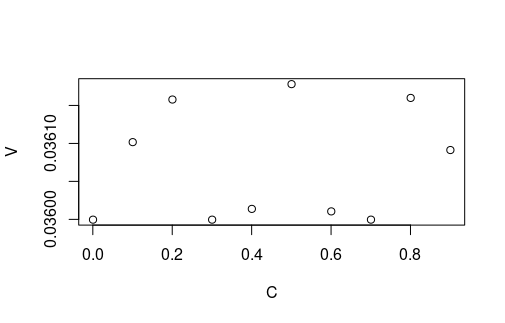
\includegraphics[width=0.5\textwidth]{grafiquito_puntos.png}}
  \subfloat[Valor de $P$ amb $\Delta t = \frac{\Delta x}{2}$]{
    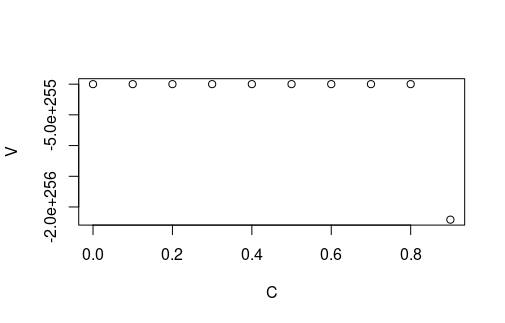
\includegraphics[width=0.5\textwidth]{puntoskk.png}}
   \caption{Gràfic del valor de $P$ en funció del temps $\Delta t$}
\end{figure}
S'observa com per a $\Delta t = \frac{\Delta x}{2}$, $P$ obté valors molt elevats  i no aproxima bé els valors reals, per contra de $\Delta t = \frac{\Delta x}{4}$ que oscil·la els valors aproximats al voltant del 0.\\\\
Concluïm doncs que el mètode amb $\Delta t = \frac{\Delta x}{2}$ no convergeix al valor real, per contra del $\Delta t = \frac{\Delta x}{4}$ que si ho fa.\\\\
Els valors obtinguts al mètode, quan  $\Delta t = \frac{\Delta x}{4}$ tenen sentit amb els resultats obtinguts a l'apartat 1 ja que estan aproximant una recta sense pendent propera al 0; pel que els valors reals deuen ser constants en el temps (resultat de l'apartat 1).
\newpage
\section{Resolució apartat 4}
Exposem ara els valors propis de la matriu definida anteriorment al programa com $A$ per als dos valors de $\Delta t$ estudiats:
\begin{figure}[h]
\captionsetup[subfigure]{labelformat=empty}
\centering
  \subfloat[Valors propis amb $\Delta t = \frac{\Delta x}{2}$]{
    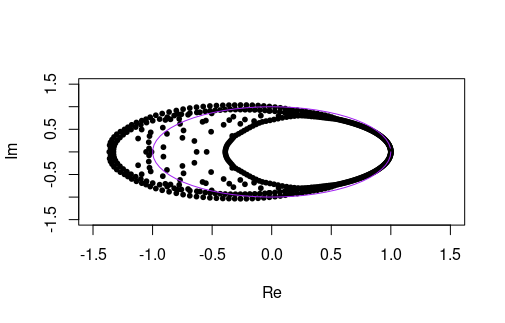
\includegraphics[width=0.5\textwidth]{partido_2.png}}
  \subfloat[Valors propis amb $\Delta t = \frac{\Delta x}{4}$]{
    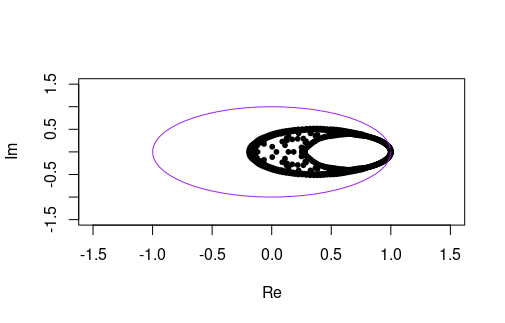
\includegraphics[width=0.5\textwidth]{partido_4.png}}
   \caption{Gràfic dels valors propis de la matrius $A$}
\end{figure}\\
S'observa com tots els valors propis de la matriu tenen norma menor a 1 si $\Delta t = \frac{\Delta x}{4}$ i que alguns son major que 1 si $\Delta t = \frac{\Delta x}{2}$.\\\\
Podem doncs conjecturar que si la norma dels valors propis de la matriu és menor o igual a 1, el mètode convergeix al valor real de la EDP, però si no es compleix la condició, el mètode no convergirà als valors reals.
\end{document}
